\section{Conceptual Model}

This chapter presents the abstract mathematical formulation of the deadly spiral phenomenon. The model consists of two interacting subsystems: continuous physiological dynamics and discrete behavioral control, forming a closed feedback loop.

\subsection{Model Abstraction and Justification}

\subsubsection{Simplifying Assumptions}

Real opioid pharmacology involves hundreds of processes. The following abstractions reduce complexity while preserving essential dynamics:

\textbf{Assumption 1: Two-compartment PK model}

\textit{Justification:} While physiologically-based models can incorporate 10+ compartments, the two-compartment model (central + peripheral) captures 90\% of concentration-time profile variance for morphine and fentanyl \cite{pharmacokinetics_textbook}. Adding more compartments increases parameter uncertainty without improving predictive accuracy for the deadly spiral phenomenon.

\textit{Validation:} Two-compartment models are standard in clinical PK studies and FDA drug approval processes.

\textbf{Assumption 2: Single metabolic pathway}

\textit{Justification:} Morphine undergoes primarily UGT2B7-mediated glucuronidation (80\% of elimination). While minor pathways exist (CYP-mediated N-demethylation), they do not exhibit significant saturation at therapeutic concentrations \cite{fentanyl_pk_2024}.

\textit{Validation:} Genetic polymorphism studies show UGT2B7 variants produce the largest PK variability, confirming its dominant role.

\textbf{Assumption 3: Aggregate tolerance}

\textit{Justification:} Cellular tolerance mechanisms (desensitization, internalization, homeostatic adaptation) operate on similar timescales (hours-days) and produce the same observable outcome (rightward EC50 shift). Modeling each separately would require 10+ additional ODEs without changing macroscopic behavior \cite{opioid_tolerance_2019}.

\textit{Validation:} Operational tolerance models successfully predict clinical dose escalation patterns \cite{tolerance_mechanisms_2018}.

\textbf{Assumption 4: Simplified pain dynamics}

\textit{Justification:} Chronic pain involves complex neuroplasticity, inflammation, and psychological factors. However, for the deadly spiral phenomenon, only the relationship between analgesia and dosing decisions matters. Pain is treated as a state variable dependent on drug effect, not an independent physiological process.

\textit{Omission justification:} Including detailed pain pathophysiology would add parameters but not change the feedback loop structure. The model's purpose is demonstrating PK-PD interaction, not pain mechanism research.

\textbf{Assumption 5: Deterministic patient}

\textit{Justification:} Real patients exhibit behavioral variability (missed doses, impulsive redosing, etc.). The model uses deterministic decision rules to isolate the systematic deadly spiral mechanism. Stochastic extensions could be added but would obscure the fundamental dynamics.

\textit{Validation:} Deterministic models successfully predict average population behavior in clinical trials \cite{pharmacodynamic_modeling}.

\subsection{Continuous Subsystem: Physiological Dynamics}

The continuous state is represented by a vector:
\begin{equation}
    \mathbf{x}(t) = [A(t), C(t), P(t), C_e(t), Tol(t)]^T \in \mathbb{R}_{\geq 0}^5
\end{equation}

\subsubsection{State Variables}

\begin{table}[H]
\centering
\caption{Continuous State Variables}
\begin{tabular}{@{}lllll@{}}
\toprule
\textbf{Symbol} & \textbf{Name} & \textbf{Domain} & \textbf{Units} & \textbf{Initial} \\ \midrule
$A(t)$ & Absorption compartment & $\mathbb{R}_{\geq 0}$ & mg & $D_0$ \\
$C(t)$ & Central concentration & $\mathbb{R}_{\geq 0}$ & mg/L & 0 \\
$P(t)$ & Peripheral concentration & $\mathbb{R}_{\geq 0}$ & mg/L & 0 \\
$C_e(t)$ & Effect-site concentration & $\mathbb{R}_{\geq 0}$ & mg/L & 0 \\
$Tol(t)$ & Tolerance factor & $[0, 3]$ & -- & 0 \\ \bottomrule
\end{tabular}
\end{table}

\subsubsection{System of Differential Equations}

The continuous dynamics follow:

\textbf{Equation 1: Absorption}
\begin{equation}
    \frac{dA}{dt} = -k_a \cdot A(t) + \sum_i D_i \cdot \delta(t - t_i)
    \label{eq:absorption}
\end{equation}
where $D_i$ are dose amounts applied at times $t_i$ (impulses from discrete subsystem).

\textbf{Equation 2: Central Compartment}
\begin{equation}
    \frac{dC}{dt} = \frac{k_a \cdot A(t)}{V_d} - \frac{V_{max} \cdot C(t)}{K_m + C(t)} \cdot \frac{1}{V_d} - k_{cp} \cdot C(t) + k_{pc} \cdot P(t)
    \label{eq:central}
\end{equation}

Terms from left to right:
\begin{enumerate}
    \item Absorption influx (first-order from gut)
    \item Metabolic elimination (Michaelis-Menten, the critical nonlinearity)
    \item Distribution to peripheral compartment
    \item Return from peripheral compartment
\end{enumerate}

\textbf{Equation 3: Peripheral Compartment}
\begin{equation}
    \frac{dP}{dt} = k_{cp} \cdot C(t) - k_{pc} \cdot P(t)
    \label{eq:peripheral}
\end{equation}

Reversible distribution between central and tissue compartments.

\textbf{Equation 4: Effect-Site Equilibration}
\begin{equation}
    \frac{dC_e}{dt} = \frac{k_{eo}}{\tau_e} \cdot (C(t) - C_e(t))
    \label{eq:effect_site}
\end{equation}

Models blood-brain barrier crossing delay. The time constant $\tau_e$ represents the hysteresis between plasma concentration and observed effect.

\textbf{Equation 5: Tolerance Development}
\begin{equation}
    \frac{dTol}{dt} = k_{in} \cdot \frac{C_e(t)}{EC_{50,signal} + C_e(t)} - k_{out} \cdot Tol(t)
    \label{eq:tolerance}
\end{equation}

Indirect response model: tolerance increases with receptor occupancy (first term) and decays slowly (second term). The ratio $k_{in}/k_{out} \approx 20$ creates asymmetric dynamics.

\subsubsection{Algebraic Output Functions}

\textbf{Analgesic Effect:}
\begin{equation}
    E(t) = 100 \cdot \frac{C_e(t)}{EC_{50}(t) + C_e(t)} \quad [\%]
    \label{eq:effect}
\end{equation}
where the tolerance-modified EC50 is:
\begin{equation}
    EC_{50}(t) = EC_{50,0} \cdot (1 + Tol(t))
    \label{eq:ec50_tolerance}
\end{equation}

This implements the rightward dose-response shift: as $Tol$ increases, higher $C_e$ is required for the same effect.

\textbf{Saturation Ratio:}
\begin{equation}
    \sigma(t) = \frac{C(t)}{K_m}
    \label{eq:saturation_ratio}
\end{equation}

Diagnostic variable characterizing elimination regime:
\begin{itemize}
    \item $\sigma < 0.5$: Linear regime (first-order kinetics)
    \item $0.5 \leq \sigma < 3$: Saturation zone (mixed-order kinetics)
    \item $\sigma \geq 3$: Plateau regime (zero-order kinetics)
\end{itemize}

\subsubsection{Phase Space Analysis}

The system exhibits two distinct dynamic regimes:

\textbf{Linear Regime ($C \ll K_m$):}

Approximating the Michaelis-Menten term as $v \approx (V_{max}/K_m) \cdot C$, the system reduces to linear ODEs with eigenvalues determined by:
\begin{equation}
    \lambda_1 = -k_a, \quad \lambda_2 = -\frac{V_{max}}{K_m \cdot V_d} - k_{cp}, \quad \lambda_3 = -k_{pc}
\end{equation}

All eigenvalues are real and negative, ensuring exponential convergence to steady-state. Periodic dosing produces stable limit cycle oscillations.

\textbf{Saturation Regime ($C \approx K_m$):}

The Michaelis-Menten nonlinearity introduces a saddle-node bifurcation. The Jacobian at equilibrium has an eigenvalue:
\begin{equation}
    \lambda_{sat} = -\frac{V_{max} \cdot K_m}{(K_m + C^*)^2 \cdot V_d}
\end{equation}

As $C^* \to \infty$, $\lambda_{sat} \to 0$, indicating loss of stability. The system exhibits slowing dynamics near the bifurcation—small perturbations cause large excursions.

\begin{figure}[H]
\centering
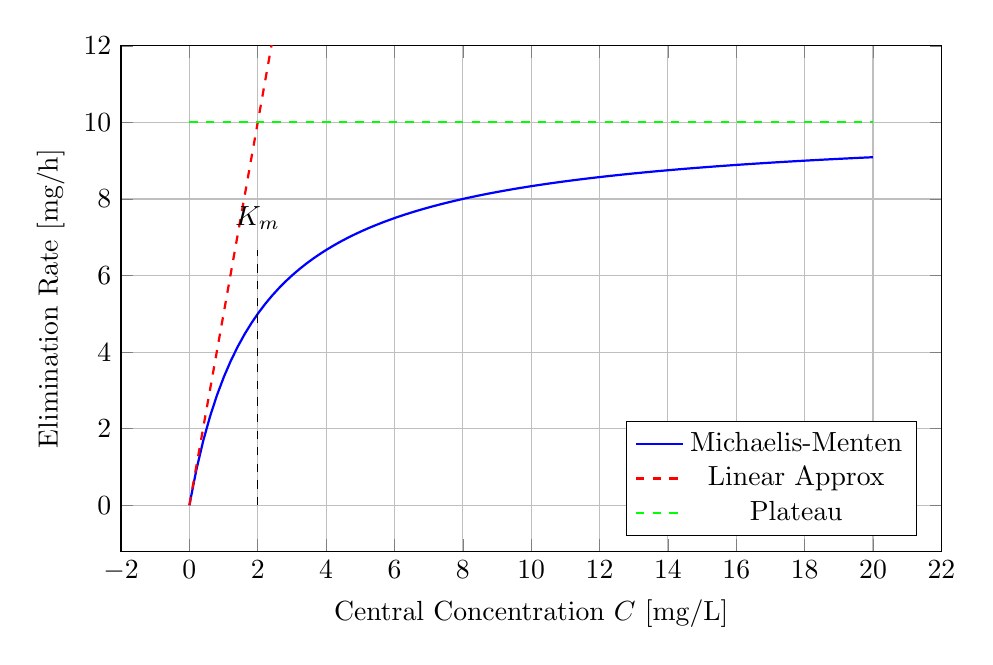
\begin{tikzpicture}
    \begin{axis}[
        width=12cm,
        height=8cm,
        xlabel={Central Concentration $C$ [mg/L]},
        ylabel={Elimination Rate [mg/h]},
        grid=major,
        legend pos=south east,
        domain=0:20,
        ymax=12
    ]
    \addplot[blue,thick,samples=100] {10*x/(2+x)};
    \addplot[red,dashed,thick] {5*x};
    \addplot[green,dashed,thick] {10};
    \legend{Michaelis-Menten, Linear Approx, Plateau}
    \draw[black,dashed] (axis cs:2,0) -- (axis cs:2,6.67);
    \node at (axis cs:2,7.5) {$K_m$};
    \end{axis}
\end{tikzpicture}
\caption{Elimination Rate vs Concentration. The transition from linear to saturated kinetics occurs near $C = K_m = 2$ mg/L. At high concentrations, elimination plateaus at $V_{max} = 10$ mg/h, creating accumulation risk.}
\label{fig:michaelis_menten}
\end{figure}

\subsection{Discrete Subsystem: Behavioral Petri Net}

The patient behavior is modeled as a condition-event Petri net with continuous state observations.

\subsubsection{Petri Net Specification}

\textbf{Places (State Variables):}

\begin{table}[H]
\centering
\caption{Petri Net Places}
\begin{tabular}{@{}llll@{}}
\toprule
\textbf{Place} & \textbf{Type} & \textbf{Domain} & \textbf{Semantics} \\ \midrule
$P_1$: Pain\_Level & Discrete & $\{0,1,2,3\}$ & Subjective pain intensity \\
$P_2$: Relief\_State & Binary & $\{0,1\}$ & Patient experiencing relief? \\
$P_3$: Motivation & Continuous & $\mathbb{R}_{\geq 0}$ & Urgency to redose \\
$P_4$: Dose\_History & Sequence & $\mathbb{N}^*$ & Log of dosing events \\
$P_5$: Time\_Counter & Continuous & $\mathbb{R}_{\geq 0}$ & Simulation time \\
$P_6$: Patient\_Alive & Binary & $\{0,1\}$ & Alive (1) or deceased (0) \\ \bottomrule
\end{tabular}
\end{table}

\textbf{Transitions (Events):}

\begin{table}[H]
\centering
\caption{Petri Net Transitions}
\begin{tabular}{@{}lll@{}}
\toprule
\textbf{Transition} & \textbf{Type} & \textbf{Trigger Condition} \\ \midrule
$T_1$: Assessment & Periodic & $t \bmod \Delta t_{assess} = 0$ \\
$T_2$: Increase\_Dose & Guarded & $P_1 \geq 2 \land P_3 > \theta_{motiv}$ \\
$T_3$: Maintain\_Dose & Guarded & $P_2 = 1 \land E(t) > \theta_{relief}$ \\
$T_4$: Detect\_Toxicity & Threshold & $C(t) > C_{toxic}$ \\
$T_5$: Administer\_Naloxone & Rescue & $T_4$ fired \\ \bottomrule
\end{tabular}
\end{table}

\subsubsection{Transition Guards and Actions}

\textbf{$T_1$: Assessment (fires every 12 hours)}

\textit{Precondition:} $P_6 = 1$ (patient alive)

\textit{Action:}
\begin{algorithmic}[1]
\State Measure $E \gets$ Effect($C_e$, $Tol$)
\If{$E < \theta_{pain,low}$}
    \State $P_1 \gets \min(P_1 + 1, 3)$
\ElsIf{$E > \theta_{pain,high}$}
    \State $P_1 \gets \max(P_1 - 1, 0)$
\EndIf
\State $P_2 \gets (E > \theta_{relief})$
\State $P_3 \gets P_3 + 0.1 \cdot P_1$
\end{algorithmic}

\textbf{$T_2$: Increase\_Dose}

\textit{Guard:} $P_1 \geq 2 \land P_3 > 1.5 \land (t - t_{last\_dose}) > 6$ hours

\textit{Action:}
\begin{algorithmic}[1]
\State $f_{esc} \gets 0.10 + 0.15 \cdot Tol(t)$ \Comment{Escalation factor}
\State $D_{new} \gets D_{current} \cdot (1 + f_{esc})$
\State $A(t) \gets A(t) + D_{new}$ \Comment{Add to absorption compartment}
\State $D_{current} \gets D_{new}$
\State $P_3 \gets P_3 - 2$ \Comment{Reset motivation}
\State Append $(t, D_{new}, C, C_e, Tol, E)$ to $P_4$
\end{algorithmic}

The escalation factor increases with tolerance, modeling the patient's unconscious self-titration.

\textbf{$T_4$: Detect\_Toxicity}

\textit{Guard:} $C(t) > C_{toxic} = 15$ mg/L

\textit{Action:}
\begin{algorithmic}[1]
\State $P_6 \gets 0$ \Comment{Patient deceased}
\State Stop simulation
\end{algorithmic}

\textbf{$T_5$: Administer\_Naloxone (optional rescue)}

\textit{Guard:} $T_4$ triggered $\land$ naloxone enabled

\textit{Action:}
\begin{algorithmic}[1]
\State $C_e(t) \gets C_e(t) \cdot 0.1$ \Comment{Competitive antagonism}
\State $P_6 \gets 1$ \Comment{Patient revived}
\State $P_3 \gets 5$ \Comment{Severe withdrawal motivation}
\end{algorithmic}

\subsubsection{Petri Net Diagram}

\begin{figure}[H]
\centering
\begin{tikzpicture}[node distance=4cm,>=stealth',bend angle=45,auto, scale=0.9, transform shape]
    \tikzstyle{place}=[circle,thick,draw=blue!75,fill=blue!20,minimum size=12mm]
    \tikzstyle{transition}=[rectangle,thick,draw=black!75,fill=black!20,minimum width=10mm,minimum height=10mm]
    
    % Places
    \node [place,tokens=2, label=above:Pain Level] (pain) {$P_1$};
    \node [place, label=above:Relief State] (relief) [right of=pain] {$P_2$};
    \node [place,tokens=1, label=left:Motivation] (motiv) [below of=pain] {$P_3$};
    
    % Transitions
    \node [transition, label=right:Assessment] (assess) [below of=relief] {$T_1$};
    \node [transition, label=left:Increase Dose] (increase) [below of=motiv] {$T_2$};
    
    % Alive place moved below Assessment to avoid collision
    \node [place,tokens=1, label=left:Patient Alive] (alive) [below of=assess] {$P_6$};
    
    % Toxicity transition
    \node [transition, label=right:Toxicity] (toxic) [right of=alive] {$T_4$};
    
    % Edges for Assessment (T1)
    \draw [->] (alive) -- (assess);
    \draw [->] (assess) -- (pain);
    \draw [->] (assess) -- (relief);
    
    % Edges for Increase Dose (T2)
    \draw [->] (pain) -- (increase);
    \draw [->] (motiv) -- (increase);
    \draw [->] (increase) to [bend right] (relief);
    
    % Edges for Toxicity (T4)
    \draw [->] (alive) -- (toxic);
    
    % Additional explanatory edges
    \draw [->, dashed] (assess) to [bend right=20] node[right, font=\small] {measure $E$} (relief);
    \draw [->, dashed] (increase) to [bend left=20] node[left, font=\small] {$A \mathrel{+{=}} D$} (motiv);
\end{tikzpicture}
\caption{Simplified Petri Net Structure. $T_1$ (Assessment) fires periodically, reading continuous state $E(t)$ to update discrete places. $T_2$ (Increase\_Dose) triggers when pain and motivation exceed thresholds, injecting a dose pulse into the continuous system. $T_4$ (Toxicity) fires when concentration exceeds safety limit, terminating the simulation.}
\label{fig:petri_net}
\end{figure}

\subsection{Hybrid System Interaction}

The deadly spiral emerges from the coupling between continuous and discrete subsystems:

\textbf{Continuous $\to$ Discrete:} Effect $E(t)$ drives pain level and relief state, determining when discrete transitions fire.

\textbf{Discrete $\to$ Continuous:} Dose events inject impulses $D \cdot \delta(t - t_i)$ into Equation \ref{eq:absorption}, perturbing the continuous trajectory.

\textbf{Feedback Loop:}
\begin{enumerate}
    \item High tolerance $\Rightarrow$ Low effect (Eq. \ref{eq:ec50_tolerance})
    \item Low effect $\Rightarrow$ High pain (Petri net $T_1$)
    \item High pain $\Rightarrow$ Dose escalation (Petri net $T_2$)
    \item Dose escalation $\Rightarrow$ Higher concentration (Eq. \ref{eq:central})
    \item If $C \approx K_m$ $\Rightarrow$ Saturation causes rapid accumulation
    \item Rapid accumulation $\Rightarrow$ Even higher tolerance (Eq. \ref{eq:tolerance})
    \item Loop back to step 1 (amplification cycle)
\end{enumerate}

\begin{figure}[H]
\centering
\begin{tikzpicture}[node distance=3cm, auto, thick, scale=1.0, transform shape]
    \tikzstyle{block} = [rectangle, draw, fill=blue!20, text width=8em, text centered, rounded corners, minimum height=4em]
    \tikzstyle{cloud} = [ellipse, draw, fill=red!20, text width=6em, text centered, minimum height=4em]
    
    \node [block] (cont) {Continuous\\ODEs};
    \node [block, right of=cont, node distance=7cm] (disc) {Discrete\\Petri Net};
    \node [cloud, below of=cont, node distance=4cm] (sat) {Saturation\\Zone};
    
    \draw [->] (cont.10) -- node[above] {$E(t), C(t)$} (disc.170);
    \draw [->] (disc.190) -- node[below] {$D_i \cdot \delta(t-t_i)$} (cont.350);
    \draw [->] (cont) -- node[left] {$C \approx K_m$} (sat);
    % Changed bend direction to right to avoid overlapping with the vertical arrow
    \draw [->, red, ultra thick] (sat) to [bend right=60] node[right, font=\bfseries] {Runaway Accumulation} (cont);
\end{tikzpicture}
\caption{Hybrid System Feedback Loop. The continuous system computes physiological state, which the discrete system observes to make dosing decisions. When concentration enters the saturation zone, the feedback loop becomes unstable, producing the deadly spiral.}
\label{fig:hybrid_loop}
\end{figure}

\subsection{Model Representation Justification}

\subsubsection{Why Differential Equations for Physiology?}

Pharmacokinetic processes are inherently continuous:
\begin{itemize}
    \item Drug molecules diffuse across membranes continuously
    \item Enzymatic reactions occur at molecular timescales ($\mu$s-ms)
    \item Blood flow distributes drug continuously
\end{itemize}

Discrete approximations (e.g., finite state machines with states Low/Medium/High concentration) would:
\begin{enumerate}
    \item Fail to capture Michaelis-Menten nonlinearity smoothly
    \item Introduce artificial state boundaries creating spurious dynamics
    \item Require arbitrarily fine discretization to approach continuous accuracy
\end{enumerate}

Differential equations are the standard representation in pharmacology \cite{pharmacokinetics_textbook} because they directly model the underlying physics.

\subsubsection{Why Petri Nets for Behavior?}

Patient decision-making is discrete:
\begin{itemize}
    \item Doses are taken at specific time points, not continuously infused
    \item Decisions have discrete outcomes (take/don't take, increase/maintain)
    \item State transitions (pain level changes) are event-driven
\end{itemize}

Alternative representations:
\begin{itemize}
    \item \textbf{Continuous approximation:} Could model dosing rate $dD/dt$, but this obscures the discrete decision structure and prevents modeling dose escalation steps.
    \item \textbf{Finite state machines:} Less expressive than Petri nets for concurrent conditions (pain $\land$ motivation $\land$ time constraints).
    \item \textbf{Agent-based models:} Overkill for single-patient simulation.
\end{itemize}

Petri nets provide the right abstraction level: expressive enough for complex decision logic, simple enough to remain analyzable \cite{petri_nets_theory}.
